% !TEX encoding = UTF-8 Unicode
\documentclass[
10pt, 
aspectratio=43, 
]{beamer}
\setbeamercovered{transparent=10}
\usetheme[
%  showheader, 
%  red, 
  purple, 
%  gray, 
%  graytitle, 
  colorblocks, 
%  noframetitlerule, 
]{Verona}

\usepackage[T1]{fontenc}
\usepackage[utf8]{inputenc}
\usepackage{lipsum}
%%%%%%%%%%%%%%%%%%%%%%%%%%%%%%%
% Mac上使用如下命令声明隶书字体, windows也有相关方式, 大家可自行修改
\providecommand{\lishu}{\CJKfamily{zhli}}
%%%%%%%%%%%%%%%%%%%%%%%%%%%%%%%
\usepackage{tikz}
\usetikzlibrary{fadings}
%
%\setbeamertemplate{sections/subsections in toc}[ball]
\usepackage{xeCJK}
\usepackage{listings}
\usepackage{caption}
\usepackage{subfigure}
\usefonttheme{professionalfonts}
\def\mathfamilydefault{\rmdefault}
\usepackage{amsmath}
\usepackage{multirow}
\usepackage{booktabs}
\usepackage{bm}
\setbeamertemplate{section in toc}{\hspace*{1em}\inserttocsectionnumber.~\inserttocsection\par}
\setbeamertemplate{subsection in toc}{\hspace*{2em}\inserttocsectionnumber.\inserttocsubsectionnumber.~\inserttocsubsection\par}
\setbeamerfont{subsection in toc}{size=\small}
\AtBeginSection[]{%
	\begin{frame}%
		\frametitle{Outline}%
		\textbf{\tableofcontents[currentsection]} %
	\end{frame}%
}

\AtBeginSubsection[]{%
	\begin{frame}%
		\frametitle{Outline}%
		\textbf{\tableofcontents[currentsection,  currentsubsection]} %
	\end{frame}%
}

\title{高等数学C}
%\subtitle{A Simple while elegant template}
\author[P.Yu]{余沛}
\mail{peiy\_gzgs@qq.com}
\institute[Guangzhou College of Technology and Business]{Guangzhou College of Technology and Business \\
  广州工商学院}
\date{\today}
\titlegraphic[width=4cm]{logo.png}{}




%%%%%%%%%%%%%%%%%%%%%%%%%%%%%%%%
% ----------- 标题页 ------------
%%%%%%%%%%%%%%%%%%%%%%%%%%%%%%%%



\begin{document}

\maketitle

%%% define code
\defverbatim[colored]\lstI{
	\begin{lstlisting}[language=C++, basicstyle=\ttfamily, keywordstyle=\color{red}]
	int main() {
	// Define variables at the beginning
	// of the block,  as in C: 
	CStash intStash,  stringStash;
	int i;
	char* cp;
	ifstream in;
	string line;
	[...]
	\end{lstlisting}
}
%%%%%%%%%%%%%%%%%%%%%%%%%%%%%%%%
% ----------- FRAME ------------
%%%%%%%%%%%%%%%%%%%%%%%%%%%%%%%%

\section{变量的极限}
\begin{frame}
	\frametitle{数列的极限与函数的极限}
	\begin{block}{定义: 数列极限与收敛数列}
		对于数列 $\{x_n\}$ 和常数 $a$, 如果有: 对于任意的 $\epsilon>0$, 都存在正整数 $N$, 使得对于任意满足 $n>N$ 的 $n$, 不等式
		$$|x_n-a|<\epsilon$$
		都成立, 
		那么称常数 $a$ 是数列 $\{x_n\}$ 的极限, 或者数列 $\{x_n\}$ 收敛, 并且收敛于 $a$, 记为
		\begin{equation*}
			\lim_{n\to\infty}x_n=a,  \quad \text{或} \quad x_n\to a (n\to\infty).
		\end{equation*}
	\end{block}
	\pause
	\begin{block}{发散数列}
		不收敛于任意常数a的数列. 
	\end{block}
	
\end{frame}
\frametitle{函数极限的性质与函数的极限}
\begin{frame}
	\begin{block}{函数极限的数列定义}
		设函数 $f(x)$ 在点 $x=a$ 的某个去心邻域内有定义, 如果存在常数 $L$, 对于任意定义在该去心邻域上收敛到$a$的数列 $\{x_n\}$, 都有 
		\begin{equation*}
			\lim_{n\to\infty} x_n = L, 
		\end{equation*}
		则称函数 $f(x)$ 在 $x=a$ 处\textbf{收敛}于 $L$, 记作 $\lim_{x \to a} f(x) = L$. 
	\end{block}
	\begin{block}{函数极限的解析定义}
		设函数 $f(x)$ 在点 $x=a$ 的某个去心邻域内有定义, 如果存在常数 $L$, 对于任意给定的正实数 $\epsilon$, 都存在正实数 $\delta$, 使得当 $0 < |x-a| < \delta$ 时, 有 $|f(x) - L| < \epsilon$ 成立, 则称函数 $f(x)$ 在 $x=a$ 处\textbf{收敛}于 $L$, 记作 $\lim_{x \to a} f(x) = L$. 
	\end{block}
\end{frame}

\section{无穷小与无穷大}

\subsection{无穷小与无穷大的概念}

\begin{frame}
	\frametitle{函数的无穷小量}
	
	
	\begin{block}{无穷小量定义}设函数 $f(x)$ 在 $x=a$ 处有定义, 如果对于任意给定的正数 $\varepsilon$, 存在正数 $\delta$, 使得当 $0 < |x-a| < \delta$ 时, 有 $|f(x)| < \varepsilon$, 则称函数 $f(x)$ 在 $x=a$ 处为无穷小量. 
	\end{block}
	\begin{itemize}
		\item<2-> \textbf{幂函数}: 当 $x$ 趋近于 $0$ 时, 函数 $f(x) = x^n$ 是无穷小量, 其中 $n$ 是正整数. \\
		\item<3-> \textbf{指数函数}: 当 $x$ 趋近于 $0$ 时, 函数 $f(x) = e^x - 1$ 是无穷小量. \\
		\item<4-> \textbf{三角函数}: 当 $x$ 趋近于 $0$ 时, 函数 $f(x) = \sin(x)$ 和 $f(x) = \tan(x)$ 是无穷小量. \\
		\item<5-> \textbf{对数函数}: 当 $x$ 趋近于 $1$ 时, 函数 $f(x) = \log(x)$ 是无穷小量. 
	\end{itemize}
	
\end{frame}

\begin{frame}
	\frametitle{函数的无穷小量}
	
	\begin{itemize}
		\item<2-> \textbf{幂函数}: 当 $x$ 趋近于 $0$ 时, 函数 $f(x) = x^n$ 是无穷小量, 其中 $n$ 是正整数. \\
		\item<3-> \textbf{指数函数}: 当 $x$ 趋近于 $0$ 时, 函数 $f(x) = e^x - 1$ 是无穷小量. \\
		\item<4-> \textbf{三角函数}: 当 $x$ 趋近于 $0$ 时, 函数 $f(x) = \sin(x)$ 和 $f(x) = \tan(x)$ 是无穷小量. 
	\end{itemize}
	\begin{figure}
		\centering
		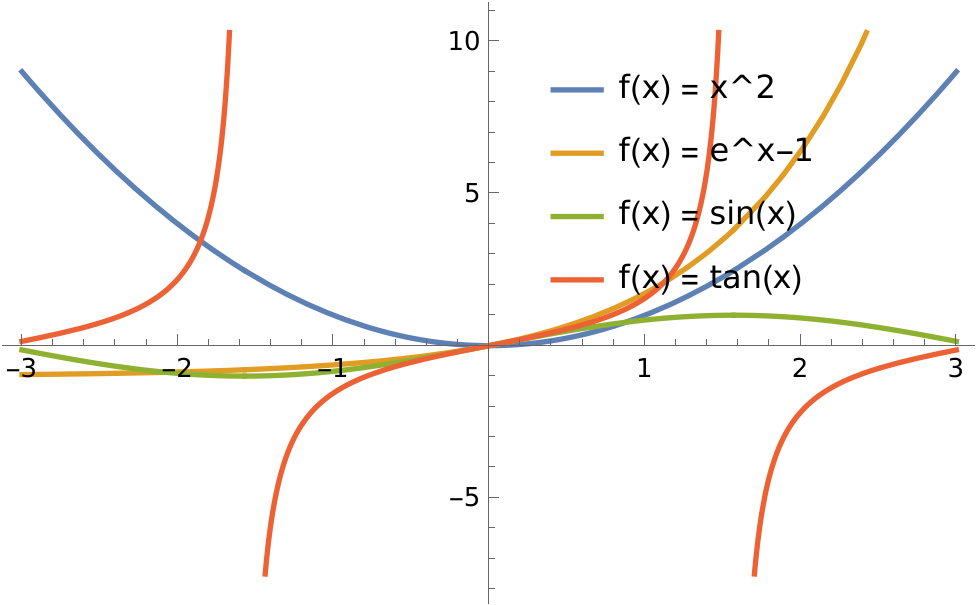
\includegraphics[width=0.5\linewidth]{small1.png}
		\caption{Enter Caption}
		\label{fig: enter-label}
	\end{figure}
\end{frame}


\begin{frame}
	\frametitle{函数的无穷小量}
	\begin{itemize}
		\item \textbf{对数函数}: 当 $x$ 趋近于 $1$ 时, 函数 $f(x) = \log(x)$ 是无穷小量. 
	\end{itemize}
	\begin{figure}
		\centering
		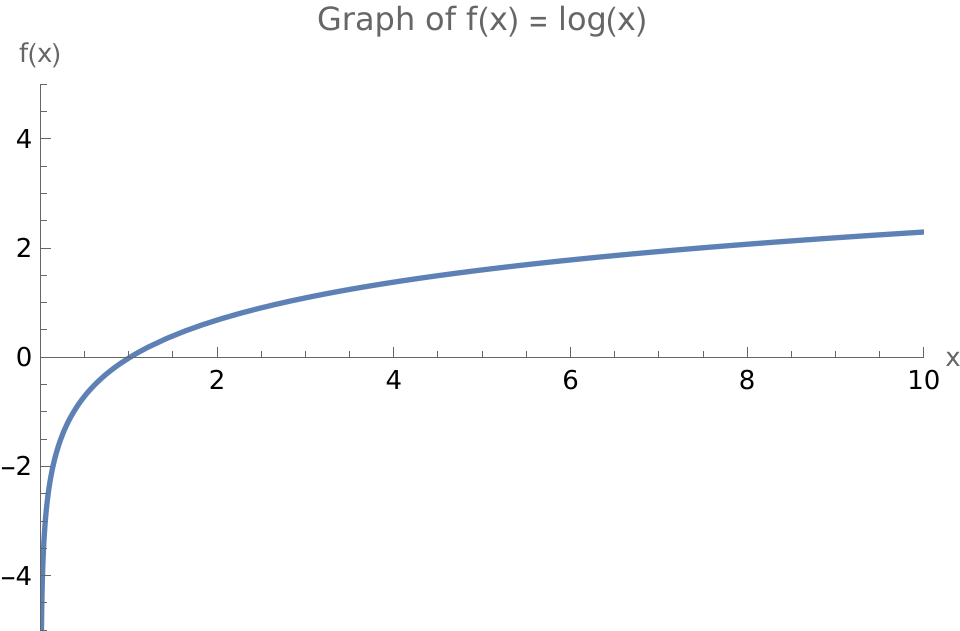
\includegraphics[width=0.5\linewidth]{log.png}
		\label{fig: enter-label}
	\end{figure}
\end{frame}


\begin{frame}
	\frametitle{函数的无穷大量}
	
	
	\begin{block}{无穷大量定义}设函数 $f(x)$ 在 $x=a$ 处有定义, 如果对于任意给定的正数 $M$, 存在正数 $\delta$, 使得当 $0 < |x-a| < \delta$ 时, 有 $|f(x)| > M$, 则称函数 $f(x)$ 在 $x=a$ 处为无穷大量. 
	\end{block}
	\begin{itemize}
		\item<1-> \textbf{幂函数}: 当 $x$ 趋近于正无穷时, 函数 $f(x) = x^n$ 是无穷大量, 其中 $n$ 是正整数. 
		\item<1-> \textbf{幂函数}: 当 $x$ 趋近于 $0$ 时, 函数 $f(x) = x^{-n}$ 是无穷大量, 其中 $n$ 是正整数. 
		\item<2-> \textbf{指数函数}: 当 $x$ 趋近于正无穷时, 函数 $f(x) = e^x$ 是无穷大量. 
		\item<4-> \textbf{对数函数}: 当 $x$ 趋近于正无穷和$0$时, 函数 $f(x) = \log(x)$ 是无穷大量. 
	\end{itemize}
\end{frame}

\begin{frame}
	\frametitle{函数的无穷大量}
	\begin{itemize}
		\item<1-> \textbf{幂函数}: 当 $x$ 趋近于正无穷时, 函数 $f(x) = x^n$ 是无穷大量, 其中 $n$ 是正整数. 
		\item<2-> \textbf{幂函数}: 当 $x$ 趋近于 $0$ 时, 函数 $f(x) = x^{-n}$ 是无穷大量, 其中 $n$ 是正整数. 
		\item<3-> \textbf{指数函数}: 当 $x$ 趋近于正无穷时, 函数 $f(x) = e^x$ 是无穷大量. 
		\item<4-> \textbf{对数函数}: 当 $x$ 趋近于正无穷和$0$时, 函数 $f(x) = \log(x)$ 是无穷大量. 
	\end{itemize}
	
	\begin{figure}
		\centering
		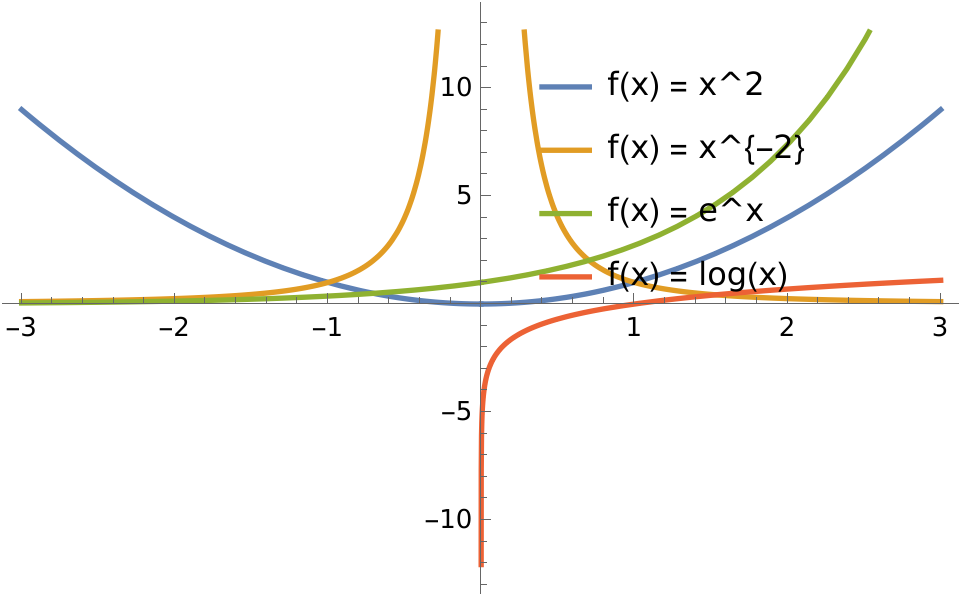
\includegraphics[width=0.5\linewidth]{infty.png}
		\label{fig: enter-label}
	\end{figure}
	
\end{frame}


\subsection{无穷小的性质}

\begin{frame}
	\frametitle{函数的无穷小量}
	
	\textbf{无穷小量的性质}: 
	\begin{itemize}
		\item 无穷小量与有限常数的乘积仍为无穷小量.\pause 
		\item 无穷小量与有界函数的乘积仍为无穷小量. \pause
		\item 无穷小量的和、差仍为无穷小量. \pause
	\end{itemize}
	
	
\end{frame}

\subsection{无穷小的比较}
\begin{frame}
	\frametitle{函数的无穷小量的比较}
	
	\begin{block}{定义: 高阶无穷小}设函数 $f(x)$ 和 $g(x)$ 在 $x=a$ 处有定义, 如果当 $x$ 趋近于 $a$ 时, 有 
		
		\[
			\lim_{x\to a}\frac{f(x)}{g(x)}=0, 
		\]
		
		则称 $f(x)$ 是 $g(x)$ 的高阶无穷小量, 记作 $f(x) = o(g(x))$. 
	\end{block}
	\pause
	\textbf{幂函数}: 当 $x$ 趋近于 $1$ 时, 幂函数 $f(x) = x^n$ ($n>1$) 是比幂函数 $g(x) = x^{n-1}$ 高阶的无穷小量, 即 $f(x) = o(g(x))$. 
	\pause
\end{frame}

\begin{frame}
	\frametitle{函数的无穷小量的比较}
	当 $x\to0$ 时,  $x,  x^2,  2 x$ 都是无穷小量,  比较它们趋向于 0 的速度, 
	\begin{itemize}
		\item $\lim _{x \rightarrow 0} \frac{x^2}{x}=0,  x^2$ 比 $x$ 要快得多; 称 $x^2$ 是比 $x$ 高阶无穷小;
		\item $\lim _{x \rightarrow 0} \frac{2 x}{x}=2, 2 x$ 与 $x$ 大致相同; 称 $2 x$ 与 $x$ 是同阶无穷小;
		\item $\lim _{x \rightarrow 0} \frac{x}{x^2}=\infty,  x$ 比 $x^2$ 要慢得多. 称 $x$ 是比 $x^2$ 较低阶无穷小. 
	\end{itemize}
	\pause
	\begin{block}{同阶无穷小}
		特别地, 如果有
		$$
		\lim \frac{\alpha}{\beta} = L, 
		$$
		则称 $\beta$ 与 $\alpha$ 是同阶无穷小量, 记作 $\alpha \sim \beta$.
	\end{block}
	\pause
	\begin{block}{等价无穷小}
		特别地, 如果有
		$$
		\lim \frac{\alpha}{\beta} = 1, 
		$$
		则称 $\beta$ 与 $\alpha$ 是等价无穷小量.
	\end{block}
\end{frame}



% Thank you page
\beamertemplateshadingbackground{structure.fg!90}{structure.fg}
\begin{frame}[plain]
	\vfill
	\centering
	{
		\centering \Huge \color{white} Thank you for your attention!\\[10pt]Questions?
		Homework:  page79:  9,  10
	}
	\vfill
\end{frame}



\end{document}

